\newpage
\quad
\newpage
\section{Relational Database Design}

\subsection{First Normal Form}
Domain is atomic if its elements are considered to be indivisible units. 

\begin{definition}
    A relational schema R is in first normal form (1NF) if the domains of all attributes of R are atomic.
\end{definition}

For the relational database, it’s required that all relations are in 1NF.

How to deal with non-atomic values:
\begin{itemize}\small
    \item For composite attributes: use a number of attributes.
    \item For multi-value attributes
    \begin{itemize}
        \item Use multi fields.
        \item Use a separate table.
        \item Use a single field.
    \end{itemize}
\end{itemize}

Drawbacks of non-atomic strategy:
\begin{enumerate}\small
    \item Complicate storage
    \item Encourage redundant storage of data
    \item Complicated to query
\end{enumerate}

Atomicity is actually a property of how the elements of the domain are used. E.g. Don't use string to store all information. 

\subsection{Pitfalls in Relational Database Design}
Relational database design requires that we find a ``good'' collection of relation schemas.

A bad design may lead to: Redundant storage, insert / delete / update anomalies --- inability to represent certain information.

\subsubsection{Decomposition}
Main refinement technique: decomposition. 
\begin{enumerate}\small
    \item All attributes of an original schema $(R)$ must appear in the decomposition $(R_1, R_2)$
    \begin{align*}
        R=R_1 \cup R_2
    \end{align*}
    \item Lossless-join decomposition (无损连接分解), i.e., for all possible relations $r$ on schema $R$
    \begin{align*}
        r=\prod_{R_1}(r)\bowtie  \prod_{R_2}(r)
    \end{align*}
\end{enumerate}

\subsubsection{Goal: Devise a Theory for the Following}
\begin{enumerate}\small
    \item Decide whether a particular relation R is in ``good'' form. --- No redundant. 
    \item In the case that a relation R is not in ``good'' form, decompose it into a set of relations ${R_1, R_2, \dots, R_n}$ such that
    \begin{itemize}
        \item Each relation is in good form.
        \item The decomposition is a lossless-join decomposition.
    \end{itemize}
\end{enumerate}

Our theory is based on:
\begin{itemize}
    \item Functional dependencies (函数依赖)
    \item Multivalued dependencies (多值依赖)
\end{itemize}

\subsection{Functional Dependencies}
\begin{definition}
    Let $R$ be a relation schema, $\alpha$ and $\beta$ be attributes, i.e. $\alpha \subset R,\ \beta \subset R$. 
    
    The functional dependency $\alpha \rightarrow \beta$ holds on $R$ if and only if for any legal relations $r(R)$, whenever any two tuples $t_1$ and $t_2$ of $r$ agree on the attributes $\alpha$, they also agree on the attributes
    \begin{align*}
        t_1[\alpha]=t_2[\alpha] \Rightarrow t_1[\beta]=t_2[\beta]
    \end{align*}
\end{definition}

$\beta$ is functionally dependent on $\alpha$, $\alpha$
functionally determines $\beta$. ($\beta$函数依赖于 $\alpha$, $\alpha$函数决定 $\beta$.)

Functional dependency --- a kind of integrity constraints, which express the relationship of values on specific attributes, can be used to judge schema normalization and to suggest refinements.

Functional dependencies allow us to express constraints that cannot be expressed using keys.

\subsubsection{The Use of Functional Dependencies}
\begin{enumerate}\small
    \item Test relations are legal under a set of  functional dependencies $F$ or not. 
    \subitem If a relation $r$ is legal under a set $F$ of functional dependencies, we say that $r$ satisfies $F$. 
    \item  Specify constraints $(F)$ on the set of legal relations --- schema. 
    \subitem We say that $F$ holds on $R$ (F在R上成立) if all legal relations $r$ on $R$ satisfy the set of functional dependencies F.
\end{enumerate}

\subsubsection{Definition of Trivial and Non-Trivial Dependency}
\begin{definition}
    A functional dependency is trivial (平凡的) if it is satisfied by all relations. In general, $\alpha\rightarrow \beta$ is trivial if $\beta \subseteq \alpha$, otherwise, is non-trivial, i.e., 
    \begin{align*}
        \text{Trivial: }& \alpha\rightarrow \beta,\text{ if }\beta \subseteq \alpha \text{ (平凡的函数依赖)}\\
        \text{Non-trivial: }&\alpha\rightarrow \beta,\text{ if }\beta \nsubseteq  \alpha \text{ (非平凡的函数依赖)}
    \end{align*}    
\end{definition}

\subsubsection{Closure of a Set of Functional Dependencies}

\begin{definition}
    The set of all functional dependencies logically implied by $F$ is the colsure of $F$ (函数依赖集$F$的闭包), denoted by $F^+$. 
\end{definition}

Armstrong’s Axioms provide inference rules to find $F^+$
\begin{enumerate}\small
    \item If $\beta \subseteq \alpha$, then $\alpha \rightarrow \beta$ (reflexivity, 自反律) --- trivial
    \item If $\alpha \rightarrow \beta$, then $\gamma \alpha\rightarrow \gamma \beta$ or $\gamma \alpha \rightarrow \beta$ (augmentation, 增补律)
    \item If $\alpha \rightarrow \beta$, and $\beta\rightarrow \gamma$, then $\alpha \rightarrow \gamma$ (transitivity, 传递律)
\end{enumerate}
These rules are 
\begin{itemize}\small
    \item [Sound] (保真的, generate only functional dependencies that actually hold)
    \item [Complete] (完备的, generate all functional dependencies that hold)
\end{itemize}

Armstrong’s Axioms additional rules
\begin{enumerate}\small
    \item If $\alpha \rightarrow \beta$ and $\alpha \rightarrow \gamma$ holds, then $\alpha \rightarrow \beta \gamma$ holds (union, 合并律)
    \item If $\alpha \rightarrow \beta\gamma$ holds, then $\alpha \rightarrow \beta$ and $\alpha \rightarrow \gamma$ holds (decomposition, 分解律)
    \item If $\alpha \rightarrow \beta$ and $\gamma \beta \rightarrow \delta$ holds, then $\alpha \gamma \rightarrow \delta$ holds (pseudo-transitivity, 伪传递律)
\end{enumerate}
The above rules can be inferred from Armstrong’s axioms.

\paragraph{Procedure for Computing \texorpdfstring{$F^+$}.}
To compute the closure of a set of functional dependencies $F$
\begin{algorithm}[H]
    \caption{Procedure for Computing $F^+$}
    \begin{algorithmic}
        \State $F^+=F$
        \Repeat
            \For{each functional dependency $f$ in $F^+$}
                \State Apply reflexivity and augmentation rules on $f$
                \State Add the resulting  to $F^+$
            \EndFor
            \For{each pair of $f_1$ and $f_2$ in $F^+$}
                \If{they can be combined using transitivity}
                    \State add the resulting  to $F^+$
                \EndIf
            \EndFor
        \Until{$F^+$ doesn't change any further}
    \end{algorithmic}
\end{algorithm}
Note: The maximum number of possible Functional Dependencies (FDs) is $2^n \times 2^n$, for $n$ attributes.

\subsubsection{Closure of Attribute Sets}

\begin{definition}
    Given a set of attributes $\alpha$, the closure of $\alpha$ under $F$ denoted by $\alpha^+$, is the set of attributes that are functionally determined by $\alpha$ under $F$ (在$F$下由$a$所直接和间接函数决定的属性的集合称为$\alpha^+$).
\end{definition}

\begin{algorithm}[H]
    \caption{To get $\alpha^+$}
    \begin{algorithmic}
        \State $result:= \alpha$
        \While{changes to result}
            \For{each $\beta \rightarrow \gamma$ in $F$}
                \If{$\beta \subseteq result$}
                    \State $result := result \cup \gamma$
                \EndIf
            \EndFor
            \State $\alpha^+ := result$
        \EndWhile
    \end{algorithmic}
\end{algorithm}

\paragraph{Uses of Attribute Set Closure}
There are 3 kind uses of the attribute set closure algorithm:
\begin{enumerate}
    \item To test $\alpha \rightarrow \beta$ is in $F^+$ $\Leftrightarrow$ $\beta \subseteq \alpha^+$
    \item To test $\alpha$ is a superkey, $\alpha \rightarrow R$ is in $F^+$ $\Leftrightarrow$ $R\subseteq \alpha^+$
    \item To compute $F^+$
    \begin{algorithm}[H]
        \caption{compute $F^+$}
        \begin{algorithmic}
            \For{each $\gamma \subseteq R$}
                \State find $\gamma^+$
                \For{each $S\subseteq \gamma^+$}
                    \State output $\gamma \rightarrow S$
                \EndFor
            \EndFor
            \State all $\gamma \rightarrow S$ form $F^+$
        \end{algorithmic}
    \end{algorithm}
    
\end{enumerate}

\subsubsection{Canonical Cover (正则覆盖)}
\begin{definition}
    Intuitively, a canonical cover of $F$, denoted by $F_c$, is a \textbf{minimal} set of FDs equivalent to $F$, i.e. no FD in $F_c$ contains an extraneous attribute. And each left side  is unique. 
    \begin{align*}
        F_c \xlongequal{\text{Logically Imply}} F
    \end{align*}
\end{definition}

To get $F_c$, we should delete extraneous attributes. There are 3 cases for the extraneous attributes:
\begin{enumerate}\small
    \item FDs can be inferred from the others
    \item redundant left side 
    \item redundant right side
\end{enumerate}

\paragraph{Extraneous Attributes (无关属性)}
Consider the FD $\alpha \rightarrow \beta$ in $F$:
\begin{enumerate}\small
    \item Attributes $A$ is extraneous in $\alpha$, if $A\in \alpha$ and $F$ logically implies $F'=(F-\left\{ \alpha\rightarrow \beta \right\})\cup \left\{ (\alpha-A)\rightarrow \beta\right\}$
    \item Attribute $A$ is extraneous in $\beta$, if $A\in \beta$ and FDs $F'=(F-\left\{ \alpha \rightarrow \beta \right\})\cup \left\{ \alpha \rightarrow (\beta - A) \right\}$ logically implies $F$. 
\end{enumerate}

\paragraph{Testing if an Attribute is Extraneous}
\begin{enumerate}\small
    \item To test $A\in \alpha$ is extraneous in $\alpha$ $\Leftrightarrow$ $\alpha=\left\{ A\alpha' \right\}$, $\left\{ A\alpha' \right\}\rightarrow \beta$, whether $\beta \in (\alpha')^+$ [$\Rightarrow \alpha\rightarrow \beta \subseteq F$]
    \item To test $A \in \beta$ is extraneous in $\beta$ $\Leftrightarrow$ $\beta=\left\{ A\beta' \right\}$, $\alpha \rightarrow \left\{ A\beta' \right\}$, whether $A\in (\alpha)^+$ [$\Rightarrow \alpha \rightarrow A \subseteq F'$, $F'=(F-\left\{ \alpha \rightarrow \beta \right\})\cup \left\{ \alpha \rightarrow (\beta - A) \right\}$]
\end{enumerate}

To compute a canonical cover for $F$:
\begin{algorithm}[H]
    \caption{compute a canonical cover}
    \begin{algorithmic}
        \Repeat
            \State Replace any FD in $F$ like $\alpha_1 \rightarrow \beta_1$ and $\alpha_1 \rightarrow \beta_2$ with $\alpha_1 \rightarrow \beta_1\beta_2$
            \State Find a FD $\alpha \rightarrow \beta$ with an extraneous attribute either in $\alpha$ or in $\beta$
            \If{an extraneous attribute is found}
                delete it 
            \EndIf
        \Until{$F$ doesn't change}
    \end{algorithmic}
\end{algorithm}

\subsection{Decomposition}

\subsubsection{Goals of Normalization}
Judge whether a relation $R$ is in a \textbf{good} form (no redundant, no insert/delete/update anomalies). If not, decompose it into a set of relations $\left\{ R_1, R_2, \dots, R_n \right\}$ such that: 
\begin{enumerate}\small
    \item a lossless-join decomposition (无损链接分解)
    \item dependency preservation (依赖保持)
    \item Each relation is in BCNF or 3NF
\end{enumerate}

\subsubsection{Desirable properties of decomposition}
\begin{enumerate}
    \item All attributes of original schema $R$ must appear in the decomposition $(R_1, R_2): R=R_1\cup R_2$
    \item Lossless-join decomposition: For all possible relations $r$ on schema $R$
    \begin{align*}
        r=\prod_{R_1}(r)\bowtie \prod_{R_2} (r)
    \end{align*}
    A decomposition of $R$ into $R_1$ and $R_2$ is lossless-join iff at least one of the following dependencies are held in $F^+$:
    \begin{itemize}\small
        \item $\left\{ R_1\cap R_2 \right\} \rightarrow R_1$
        \item $\left\{ R_1\cap R_2 \right\} \rightarrow R_2$
    \end{itemize}
    (分解后的二个子模式的共同属性必须是$R_1$或$R_2$的码(适用于一分为二的分解))
    \item Dependency preservation: Restriction of $F$ to $R_i$ is : $F_i\subseteq F^+$, $F_i$ includes only attributes of $R_i$. 
    \begin{align*}
        (F_1\cup F_2\cup\cdots\cup F_n)=F^+
    \end{align*}
    where $F_i$ be the set of dependencies in $F^+$ that include only attributes in $R_i$. 
    \item No redundancy: $R_i$ should be in BCNF or 3NF. 
\end{enumerate}

\subsubsection{Testing for Dependency Preservation}

\begin{algorithm}[H]
    \caption{check $\alpha \rightarrow \beta$ is preserved in a decomposition}
    \begin{algorithmic}
        \State $result=\alpha$
        \While{changes to $result$}
            \For{$R_i$ in the decomposition}
                \State $t=(result\cap R_i)^+ \cap R_i$
            \EndFor
            \State $result=result\cup t$
            \If{$result$ contains all attributes in $\beta$}
                \State $\alpha \rightarrow \beta$ is preserved
            \EndIf
        \EndWhile
    \end{algorithmic}
\end{algorithm}
Apply the test on all dependencies in F to check if a decomposition is dependency preserving.


对于$F$中的某个$\alpha\rightarrow\beta$, 投影到各个$R_i$中, 判别是否有某个$R_i$能保持函数依赖$\alpha\rightarrow\beta$. 若对$F$中的每个$\alpha\rightarrow\beta$都能有一个$R_i$满足函数依赖, 则该分解保持依赖.

\subsection{Boyce-Codd Normal Form}
\begin{definition}
    A relation schema $R$ is in BCNF, with respect to a set $F$ of FDs, if $\forall$ FDs in $F^+$ of the form $\alpha \rightarrow \beta$, where $\alpha \subseteq R$ and $\beta \subseteq R$, at least one of the following holds: $\forall \alpha \rightarrow \beta$ in $F^+$, 
    \begin{align*}
        \left\{\begin{array}{rl}
            & \alpha\rightarrow \beta \text{ is trivial }(\text{i.e. }\beta \subseteq \alpha)\\
            \text{or }&\alpha \text{ is a superkey for } R (\text{i.e. } R\subseteq \alpha^+,\ \alpha \rightarrow R)
        \end{array}\right.
    \end{align*}
\end{definition}

\subsubsection{Testing for BCNF}
To check if a non-trivial dependency $\alpha\rightarrow\beta$ causes a violation of BCNF
\begin{enumerate}\small
    \item Compute $\alpha^+$
    \item Verify that $\alpha^+$ includes all attributes of $R$ ($\alpha$ os a superkey of $R$)
\end{enumerate}

To check if a relation schema $R$ is in BCNF, it suffices to check only the dependencies in the given set $F$ for violation of BCNF. However, using only $F$ to test for BCNF may be incorrect when testing a relation $R_i$ in a decomposition of $R$.

可在$F$下判别$R$是否违反BCNF, 但必须在$F^+$下判别$R$的分解式是否违反BCNF.


\subsubsection{BCNF Decomposition Algorithm}
\begin{algorithm}[H]
    \caption{BCNF Decomposition Algorithm}
    \begin{algorithmic}
        \State $result:=\left\{ R \right\}$
        \State $done:=false$
        \While{not $done$}
            \If{there is a schema $R_i$ in $result$ that is not in BCNF}
                \State let $\alpha\rightarrow \beta$ be a non-trivial FD that holds on $R_i$ such that $\alpha \rightarrow R_i$ is not in $F^+$, and $\alpha \cap \beta =\emptyset$
                \State $result:=(result - R_i) \cup \underbrace{(\alpha, \beta)}_{R_{i1}} \cup \underbrace{(R_i-\beta)}_{R_{i2}} $ \Comment 将$R_i$分解为二个子模式: $R_{i1}, R_{i2}$, $\alpha$是 它们的共同属性.
            \Else 
                \State $done:=true$
            \EndIf
        \EndWhile
    \end{algorithmic}
\end{algorithm}
Finally, every sub-schema is in BCNF, and the decomposition is lossless-join.

\subsubsection{BCNF and Dependency Preservation}
It is not always possible to get a BCNF decomposition that is dependency preserving. Therefore, we cannot always satisfy all three design goals:
\begin{enumerate}\small
    \item Lossless-join
    \item BCNF
    \item Dependency preservation
\end{enumerate}

\subsection{Third Normal Form}
A weaker normal form: 
\begin{enumerate}\small
    \item Allows some redundancy (with resultant problems).
    \item But FDs can be checked on individual relations without computing a join --- dependency preserving.
    \item There is always a lossless-join, dependency preserving decomposition into 3NF.
\end{enumerate}

\subsubsection{Third Normal Form (3NF)}
\begin{definition}
    A relation schema $R$ is in third normal form (3NF) if $\forall\ \alpha \rightarrow \beta$ in $F^+$, at least one of the following conditions holds:
    \begin{itemize}\small
        \item $\alpha \rightarrow \beta$ is trivial (i.e., $\beta \in \alpha$)
        \item $\alpha$ is a superkey for $R$
        \item Each attribute $A$ in $\beta -\alpha$ is contained in a candidate key for $R$ (即$A\in \beta-\alpha$是主属性, 若$\alpha \cap \beta =\emptyset$, 则$A=\beta$是主属性)
    \end{itemize}
\end{definition}
Note: each attribute may be in a different candidate key.

If a relation is in BCNF, it is in 3NF. Third condition is a minimal relaxation of BCNF to ensure dependency preservation. 

\paragraph{Redundancy of 3NF}
A schema that is in 3NF but not in BCNF has the problems of repetition of information, and may need to use null values. 

\subsubsection{Testing for 3NF}
\begin{enumerate}
    \item  Need to check only FDs in $F$, need not check all FDs in $F^+$.
    \item Use attribute closure to check for each dependency $\alpha\rightarrow\beta$, to see if $\alpha$ is a superkey.
    \item If $\alpha$ is not a superkey, we have to verify if each attribute in $\beta$ is contained in a candidate key of $R$. (This test is rather more expensive, since it involve finding all candidate keys)
\end{enumerate}

\subsubsection{Comparison of BCNF and 3NF}
It is always possible to decompose a relation into relations in 3NF and
\begin{itemize}\small
    \item The decomposition is lossless.
    \item The dependencies are preserved.
\end{itemize}

It is always possible to decompose a relation into relations in BCNF and
\begin{itemize}\small
    \item The decomposition is lossless.
    \item But it may not be possible to preserve dependencies.
\end{itemize}

\subsubsection{3NF Decomposition Algorithm}

\begin{algorithm}[H]
    \caption{3NF Decomposition Algorithm}
    \begin{algorithmic}
        \State Let $F_c$ be a canonical cover for $F$
        \State $i:=0$
        \For{each FD $\alpha \rightarrow \beta$ in $F_c$}
            \If{none of the schemas $R_j$, $1\le j\le i$ contains $\alpha\beta$}
                \State $i:=i+1$
                \State $R_i=(\alpha\beta)$
                \Comment 将$F_c$中的每个$\alpha \rightarrow \beta$ 分解为子模式$R_i := (\alpha, \beta)$, 从而保证dependency-preserving.
            \EndIf
        \EndFor
        \If{none of the schemas $R_j$, $1\le j \le i$ contains a candidate key for $R$}
            \State $i:=i+1$
            \State $R_i:=$ any candidate key for $R$ 
            \Comment 保证至少在一个$R_i$中存在$R$的候选码, 从而保证lossless-join.
        \EndIf
        \State \Return{$(R_1, R_2, \dots, R_i)$}
    \end{algorithmic}
\end{algorithm}


\subsubsection{Design Goals}
Goal for a relational database design is:
\begin{itemize}\small
    \item BCNF.
    \item Lossless join.
    \item Dependency preservation.
\end{itemize}

If we cannot achieve this, we accept one of
\begin{itemize}\small
    \item Lack of dependency preservation.
    \item Redundancy due to use of 3NF.
\end{itemize}

\subsection{Multivalued Dependencies}
\subsubsection{Multivalued Dependencies (MVDs)}
\begin{definition}
    Let $R$ be a relation schema and let $\alpha \subseteq R$ and $\beta \subseteq R$, the multivalued dependency 
    \begin{align*}
        \alpha \rightarrow \rightarrow \beta
    \end{align*}
    holds on $R$, if in any legal relation $r(R)$, $\forall$ pairs of tuples $t_1$ and $t_2$ in $r$ such that $t_1[\alpha]=t_2[\alpha]$, there exist tuples $t_3$ and $t_4$ in $r$ such that: 
    \begin{align*}
        t_1[\alpha]&=t_2[\alpha]=t_3[\alpha]=t_4[\alpha]\\
        t_3[\beta]&=t_1[\beta]\\
        t_4[\beta]&=t_2[\beta]\\
        t_3[R-\alpha-\beta]&=t_2[R-\alpha-\beta]\\
        t_4[R-\alpha-\beta]&=t_1[R-\alpha-\beta]
    \end{align*}
\end{definition}

If $\beta \subseteq \alpha$ or $\alpha \cup \beta=R$, then $\alpha\rightarrow\rightarrow\beta$ is trivial. 

\begin{table}[H]
    \centering
    \caption{Tabular representation of $\alpha\rightarrow\rightarrow\beta$}
    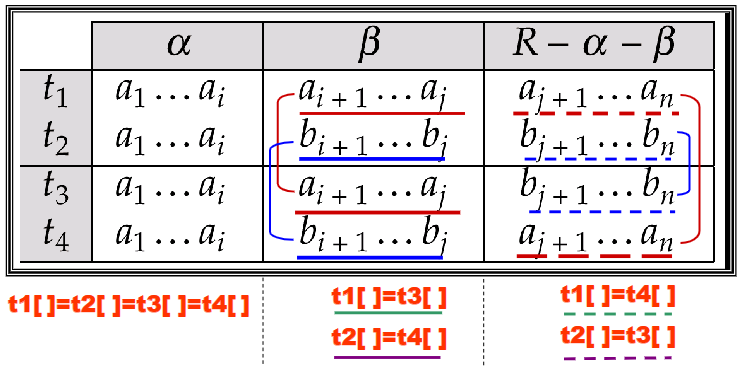
\includegraphics[width=0.42\textwidth]{DB6/Multivalued Dependencies}
\end{table}

\subsubsection{Theory of MVDs}
If $\alpha\rightarrow\beta$, then $\alpha\rightarrow\rightarrow\beta$ (If $R-\alpha-\beta=\emptyset$, i.e., $\alpha\cup \beta=R$). That is, every FD is also a multivalued dependency.

The closure $D^+$ of $D$ is the set of all functional and multivalued dependencies logically implied by $D$.
\begin{itemize}\small
    \item We can compute $D^+$ from $D$, using the formal definitions of FDs and multivalued dependencies.
    \item We can manage with such reasoning for very simple multivalued dependencies, which seem to be most common in practice.
    \item For complex dependencies, it is better to reason about sets of dependencies using a system of inference rules. 
\end{itemize}

\subsection{Fourth Normal Form}
\begin{definition}
    A relation schema $R$ is in 4NF with respect to a set $D$ of functional and multivalued dependencies if $\forall$ multivalued dependencies in $D^+$ of the form $\alpha\rightarrow\rightarrow\beta$, where $\alpha\subseteq R$ and $\beta\subseteq R$,at least one of the following hold:
    \begin{itemize}\small
        \item $\alpha\rightarrow\rightarrow\beta$ is trivial (i.e., $\beta\subseteq\alpha$ or $\alpha\cup \beta=R$)
        \item $\alpha$ is a superkey for schema $R$. 
    \end{itemize}
\end{definition}
If a relation is in 4NF, it is in BCNF.

\subsubsection{Requirement for decomposition --- Restriction of Multivalued Dependencies}
Assume $R$ is decomposed into $R_1, R_2, \dots, R_n$, each $R_i$ is required to conform to 4NF. The restriction of $D$ to $R_i$ is the set $D_i$ consisting of 
\begin{itemize}\small
    \item All functional dependencies in $D^+$ that include only attributes of $R_i$. 
    \item All multivalued dependencies of the form
    \begin{align*}
        \alpha \rightarrow \rightarrow (\beta\cap R_i)
    \end{align*}
    where $\alpha\subseteq R_i$ and $\alpha \rightarrow\rightarrow\beta$ is in $D^+$. 
\end{itemize}

\subsubsection{4NF Decomposition Algorithm}
\begin{algorithm}[H]
    \caption{4NF Decomposition Algorithm}
    \begin{algorithmic}
        \State $result:=\left\{R\right\}$
        \State $done=false$
        \State compute $D^+$
        \State Let $D_i$ denote the restriction of $D^+$ to $R_i$. 
        \While{not $done$}
            \If{there is a schema $R_i$ in $result$ that is not in 4NF}
                \State Let $\alpha\rightarrow\rightarrow \beta$ be a non-trivial multivalued dependency that holds on $R_i$ such that $\alpha\rightarrow R_i$ is not in $D_i$, and $\alpha \cap \beta =\emptyset$. 
                \State $result:=(result-R_i)\cup\underbrace{(\alpha, \beta)}_{R_{i1}}\cup\underbrace{(R_i-\beta)}_{R_{i2}}$
            \EndIf
        \EndWhile
    \end{algorithmic}
\end{algorithm}
Note: each $R_i$ is in 4NF, and decomposition is lossless-join.

\subsubsection{Other Design Issues}
Some aspects of database design are not caught by normalization.
